\documentclass[conference]{IEEEtran}
\IEEEoverridecommandlockouts

% no hyperref: lecturer wants hyperlinks deactivated
\usepackage{graphicx}
\usepackage{subcaption}
\usepackage{booktabs}
\usepackage{url}
\usepackage{amsmath}
\usepackage{amssymb}
\usepackage{array}
\usepackage{cite}          % sorted, compressed numeric citations
\usepackage{algorithm}
\usepackage{algpseudocode}
\usepackage{fancyhdr}

\pagestyle{fancy}
\fancyhf{}
\cfoot{\thepage}
\renewcommand{\headrulewidth}{0pt}

\begin{document}

\title{Option 1: Training Neural Networks on Mini-Batches with Static and
Dynamic Particle Swarm Optimisation}

\author{\IEEEauthorblockN{Gabriella Scott}
\IEEEauthorblockA{Student number: 25935453\\
Email: 25935453@sun.ac.za}}

\maketitle

\begin{abstract}
Mini-batch training of a neural network evaluates the error on a
different subset of the data at every step, so the error surface
changes over time. Neural network training under mini-batching is
therefore a dynamic optimisation problem. This study tested the
hypothesis that an optimiser developed for dynamic problems is the best
choice to train neural networks under mini-batching. Stochastic
gradient descent, a static inertia particle swarm optimiser and a
dynamic quantum-inspired particle swarm optimiser were compared on three
classification problems with five batch sizes. The quantum particle
swarm optimiser significantly outperformed the static particle swarm
optimiser under mini-batching, and the difference disappeared with
full batch. Stochastic gradient descent still produced the best
results overall. The hypothesis was therefore only partly supported.
\end{abstract}

% ============================================================
\section{Introduction}
Training a feedforward neural network (NN) is an optimisation problem,
where the goal is to find the weights that minimise an error function
\cite{engelbrecht2007}. The standard approach uses stochastic
gradient descent (SGD) on mini-batches, where every weight update uses
the error on a small random subset of the training data
\cite{dennis2021}. Dennis \textit{et al.} showed that the error
surface changes when the subset changes, and concluded that
mini-batch training is a dynamic optimisation problem
\cite{dennis2021}.

The assignment hypothesis follows from the conclusion of Dennis
\textit{et al.}: an optimisation algorithm developed for dynamic
problems is the best choice to train an NN when mini-batches are used.
This study tested the hypothesis using three training algorithms. SGD was 
used as the baseline, while the quantum-inspired particle swarm optimiser 
(QSO) was used as the dynamic algorithm. The standard inertia particle swarm 
optimiser (PSO) provided a static control to determine whether the dynamic 
mechanisms of QSO affected performance. The algorithms were evaluated on 
three classification problems across five batch sizes, using networks with 
weight decay and 30 independent runs per configuration.

The remainder of the report is organised as follows.
Section~\ref{sec:background} gives the background on NNs, PSO and
dynamic optimisation. Section~\ref{sec:impl} describes the
implementation, and Section~\ref{sec:emp} describes the empirical
process. Section~\ref{sec:results} presents and discusses the results.
Section~\ref{sec:concl} concludes the report.

% ============================================================
\section{Background}
\label{sec:background}
This section gives the background needed to follow the study.
Feedforward NNs, gradient-based training with mini-batches and weight
decay are described first. PSO and the problems that PSO faces in
dynamic environments are then discussed, including the QSO. The
section ends with the evidence that NN training under mini-batching
is a dynamic optimisation problem.

\subsection{Feedforward Neural Networks}
A feedforward NN with one hidden layer maps $I$ inputs to $K$
outputs through $H$ hidden units. Each hidden unit computes a
weighted sum of the inputs plus a bias. The sum is passed through the
sigmoid function $\sigma(a) = 1/(1 + e^{-a})$, also known as the
logistic function \cite{kelleher2015}. Each output unit
computes a weighted sum $a_k$ of the hidden unit outputs plus a bias.
For classification with $K$ classes, a softmax output layer converts
the sums into class probabilities \cite{dennis2021},
\begin{equation}
o_k = \frac{e^{a_k}}{\sum_{m=1}^{K} e^{a_m}}.
\end{equation}
All weights and biases together form the weight vector
$\boldsymbol{\theta}$ of $n_x = H(I+1) + K(H+1)$ elements.

The error of the network on a set $B$ of training patterns is measured
with the cross-entropy \cite{dennis2021},
\begin{equation}
E(\boldsymbol{\theta}, B) = -\frac{1}{|B|} \sum_{p \in B}
\sum_{k=1}^{K} d_{k,p} \ln o_{k,p},
\label{eq:ce}
\end{equation}
where $o_{k,p}$ is the output of unit $k$ for pattern $p$, and
$d_{k,p}$ is one if pattern $p$ belongs to class $k$ and zero
otherwise. Training searches for the weight vector that minimises the
error, so NN training is an optimisation problem
\cite{engelbrecht2007}.

\subsection{Gradient Descent and Mini-Batch Training}
Gradient descent starts from random weights and repeatedly takes a
small step downhill on the error surface
\cite{kelleher2015}. The weight update is
\begin{equation}
\boldsymbol{\theta}(t+1) = \boldsymbol{\theta}(t)
- \alpha \nabla f(\boldsymbol{\theta}(t)),
\end{equation}
where $t$ is the time step, $f$ is the objective function and $\alpha$
is the learning rate. A small learning rate converges slowly, and a
large learning rate makes the weights jump across the error surface
\cite{kelleher2015}. For NNs, the gradient is computed
with backpropagation, and gradient descent with backpropagation is the
best-known NN training algorithm \cite{dennis2021}.

Batch gradient descent calculates the gradient over the entire training set 
and makes one weight update per pass \cite{kelleher2015}. Mini-batch 
training instead divides the training set into random subsets, updating the 
weights after each subset \cite{dennis2021}. A complete pass through the 
training set is called an epoch. Each update therefore uses the error from 
a small subset as an estimate of the error across the full training set. In 
this report, gradient descent using mini-batches is referred to as SGD.

\subsection{Weight Decay}
A network with more hidden units than needed can fit the noise in the
training data and generalise poorly. Weight decay limits this
overfitting by adding a penalty on large weights to the error
\cite{goodfellow2016}. The objective function becomes
\begin{equation}
f(\boldsymbol{\theta}) = E(\boldsymbol{\theta}, B)
+ \frac{\lambda}{2} \sum_{j} \theta_j^2,
\label{eq:obj}
\end{equation}
where the sum runs over the weights, excluding the biases, and
$\lambda$ is the penalty coefficient. Goodfellow \textit{et al.}
explained that weight decay shrinks the weight components that do not
help to reduce the error, and that the biases are normally left
un-penalised \cite{goodfellow2016}. A larger $\lambda$ gives stronger
regularisation, and the best value has to be found through
experiments with different values \cite{goodfellow2016}.

\subsection{Particle Swarm Optimisation}
PSO is a population-based search algorithm based on the social
behaviour of birds in a flock \cite{engelbrecht2007}. A swarm of $n_s$ particles moves through an $n_x$-dimensional search
space \cite{engelbrecht2007}. Each particle $i$ has a
position $\mathbf{x}_i(t)$, a velocity $\mathbf{v}_i(t)$ and a
personal best position $\mathbf{y}_i(t)$, the best position that the
particle has visited. In the global best (gbest) PSO, 
$\hat{\mathbf{y}}(t)$ is the best personal best position of the swarm
\cite{engelbrecht2007}. With an inertia weight $w$, the
velocity in dimension $j$ is updated as
\begin{equation}
\begin{split}
v_{ij}(t+1) = {} & w v_{ij}(t) + c_1 r_{1j}(t)[y_{ij}(t) - x_{ij}(t)] \\
& + c_2 r_{2j}(t)[\hat{y}_j(t) - x_{ij}(t)],
\end{split}
\end{equation}
and the position as
$\mathbf{x}_i(t+1) = \mathbf{x}_i(t) + \mathbf{v}_i(t+1)$
\cite{engelbrecht2007}. The acceleration coefficients
$c_1$ and $c_2$ scale the pull towards the personal best and the
global best positions, and $r_{1j}(t), r_{2j}(t) \sim U(0,1)$. The
inertia weight controls how much of the previous velocity is kept,
and therefore the balance between exploration and exploitation
\cite{engelbrecht2007}. A personal best position is replaced
when the new position has a lower value of $f$
\cite{engelbrecht2007}.

To train an NN with PSO, each particle represents one complete
network, so each element of the position is one weight or bias
\cite{engelbrecht2007}. The objective function of
\eqref{eq:obj} serves as the fitness function. PSO only needs the
value of $f$ and uses no gradient information.

\subsection{Dynamic Optimisation Problems}
In a dynamic optimisation problem, the quality of a solution changes over 
time \cite{dennis2021}. Engelbrecht identified two reasons why standard PSO 
struggles in these environments \cite{engelbrecht2007}. The first is outdated 
memory. After a change, the personal best and global best positions still contain 
fitness values from before the change. If the stored global best is better 
than the values found after the change, the swarm remains attracted to the 
old optimum. Reevaluating the personal best positions after a change can 
address this problem. The second reason is loss of diversity. As the swarm converges, the particles 
move closer to the global best and their velocities approach zero. This makes 
it difficult for the swarm to find an optimum that has moved outside the 
contracted swarm. Engelbrecht identified diversity loss as the main cause of 
PSO failure in dynamic environments \cite{engelbrecht2007}.

Blackwell and Branke addressed diversity loss with quantum particles
\cite{blackwell2006}. The QSO splits the swarm into neutral particles,
which follow the normal PSO updates, and quantum particles. A quantum
particle has no velocity. At every time step, the position of a
quantum particle is sampled uniformly from $B_{\hat{\mathbf{y}}}(r_{cloud})$,
a hypersphere of radius $r_{cloud}$ around the global best position,
called the quantum cloud. The
neutral particles refine the current best solution, while the quantum
particles keep searching close to the best solution. The idea follows
the atomic swarm of the charged PSO, in which half of the particles
repel each other to maintain diversity
\cite{engelbrecht2007}. Blackwell and Branke combined
the quantum particles with multiple swarms, whereas this study used a
single swarm with re-evaluation of the personal best positions.

\subsection{Neural Network Training as a Dynamic Problem}
Dennis \textit{et al.} used fitness landscape analysis to investigate how 
the NN error surface changes when the error is calculated on subsets of the 
data \cite{dennis2021}. Since the error in \eqref{eq:ce} depends on the 
patterns in $B$, the same weight vector can have a different error for each 
mini-batch. Dennis \textit{et al.} found significant differences in 
characteristics such as ruggedness, searchability and modality between 
subsets, with these differences occurring more often for smaller batches. 
They also found that the minima of a subset did not reliably predict the 
location of the minima on the full data set. Based on these findings, 
Dennis \textit{et al.} concluded that training on changing subsets can be 
viewed as a dynamic optimisation problem. They suggested investigating 
dynamic optimisation algorithms for NN training, which motivates this study.

In summary, mini-batch training changes the error surface at every
step, and PSO needs mechanisms such as re-evaluation and quantum
particles to handle such changes.

% ============================================================
\section{Implementation}
\label{sec:impl}
This section describes how the network and the three training
algorithms were implemented. The network and the objective function
are described first, followed by the training algorithms. All code
was written in Python~3.10 and is available in a public Git
repository\footnote{\url{https://github.com/Gabriella-Scott/ML_Assignments/tree/main/Assignment3}}.
The network, SGD, PSO and QSO were implemented from scratch with
NumPy. Scikit-learn was used only to load the data sets, to split the
data and to compute the accuracy and the F1 score. SciPy provided the statistical
tests. Every run used a fixed random seed, so every result can be
reproduced.

\subsection{Neural Network and Objective Function}
The weight vector $\boldsymbol{\theta}$ was stored as a flat array 
containing $n_x$ elements. During the forward pass, it was reshaped into a 
hidden layer matrix and an output layer matrix, with the biases stored in 
the last column of each matrix. The entire mini-batch was then processed 
using two matrix multiplications. In \eqref{eq:obj}, a mask vector containing 
zeroes for the bias terms was used to exclude the biases from the penalty.

The gradient for SGD was computed with backpropagation. The gradient
was checked against central finite differences on randomly chosen
weights. The largest relative difference was below $10^{-8}$, which
confirmed the backpropagation code.

\subsection{Training Algorithms}
A batch generator shuffled the training set at the start of every
epoch and returned the next mini-batch on request. With full batch,
the generator always returned the whole training set. SGD made one
weight update per mini-batch, without momentum.

PSO and QSO used the same training loop. At each iteration, the loop selected 
the next mini-batch, evaluated all particles on it, updated the personal and 
global best positions, and then moved the particles. QSO was implemented as a 
subclass of PSO that overrides two steps, as shown in Algorithm~\ref{alg:qso}.

The first step handles a new mini-batch. QSO re-evaluated all personal best 
positions on the new mini-batch and recalculated the global best, while PSO 
kept the stored values. The second step moves the particles. Neutral particles 
used the standard velocity and position updates, while each quantum particle 
was given a random direction from a normalised Gaussian vector. It was then 
placed at a distance of $r_{cloud} u^{1/n_x}$ from the global best position, 
where $u \sim U(0,1)$. This scaling distributes the samples uniformly 
throughout the volume of the hypersphere.

\begin{algorithm}[t]
\caption{Quantum-inspired particle swarm optimisation for mini-batch training}
\label{alg:qso}
\begin{algorithmic}[1]
\State Create and initialise a swarm of neutral and quantum particles
\Repeat
  \State Draw the next mini-batch
  \State Re-evaluate every personal best position on the new mini-batch
  \State Set the global best position to the best personal best position
  \For{each particle}
    \State Evaluate the current position on the mini-batch
    \State Update the personal best and global best positions
  \EndFor
  \For{each neutral particle}
    \State Update the velocity and the position
  \EndFor
  \For{each quantum particle}
    \State Sample a new position uniformly within the quantum cloud
    \Statex \hspace{\algorithmicindent}\hspace{\algorithmicindent}around the global best position
  \EndFor
\Until{the budget is used}
\State \Return the global best position
\end{algorithmic}
\end{algorithm}

A counter recorded the number of pattern presentations used by every
evaluation, including the re-evaluations of QSO. Training stopped when
the budget was used. SGD returned the final weight vector, and the
swarms returned the global best position.

In summary, all three algorithms shared the same network code,
objective function, batch generator and budget counter, so the
algorithms differed only in how the weights were updated.

% ============================================================
\section{Empirical Process}
\label{sec:emp}
This section describes how the experiments were set up so that the
three training algorithms were compared fairly. The classification
problems and the pre-processing are described first, followed by the
mini-batch sizes, the architecture and the regularisation. The control
parameters and the training budget are then given. The section ends
with the performance measures and the statistical analysis.

\subsection{Classification Problems and Pre-Processing}
Three classification problems were used, namely Iris, Wine and breast
cancer Wisconsin (diagnostic). All three data sets were loaded with
the dataset functions of
scikit-learn\footnote{\url{https://scikit-learn.org/stable/datasets/toy_dataset.html}}.
Table~\ref{tab:data} summarises the problems. The problems differ in
the number of inputs and classes, and Wine and breast cancer have
imbalanced classes.

\begin{table}[t]
\centering
\caption{Classification problems and network sizes}
\label{tab:data}
\small
\setlength{\tabcolsep}{3pt}
\begin{tabular}{lccccc}
\toprule
Problem & Inputs & Class sizes & Hidden & Weights & $\lambda$ \\
\midrule
Iris          & 4  & 50/50/50 & 10 & 83  & $10^{-3}$ \\
Wine          & 13 & 59/71/48 & 20 & 343 & $10^{-4}$ \\
Breast cancer & 30 & 212/357  & 20 & 662 & $10^{-3}$ \\
\bottomrule
\end{tabular}
\end{table}

Each run split the data into a training set (60\%), validation set (20\%), and 
test set (20\%). The validation set was used only for parameter selection and 
convergence plots, while the test set was reserved for the final 
results \cite{kelleher2015}. The split was stratified to preserve the class 
proportions across all three subsets. A different random split was used for 
each of the 30 runs.

All inputs were standardised to have a mean of zero and a standard deviation
of one. Kelleher \textit{et al.} noted that large differences in input 
ranges can make learning more difficult, and the Wine dataset contains 
features with very different ranges \cite{kelleher2015}. The mean and 
standard deviation were calculated from the training set only and then 
applied to the validation and test sets. This prevented information from the 
test set from leaking into training. The class labels were one-hot encoded to 
match the softmax output layer.

\subsection{Mini-Batch Sizes}
Five batch sizes were used: eight, 16, 32 and 64 patterns, and the
full training set. The mini-batch sizes are powers of two and range
from very small to large relative to the training sets of 90 to 341
patterns. Dennis \textit{et al.} used window sizes of 50, 100 and 150, which 
corresponds to batch sizes \cite{dennis2021}. 
Sizes of eight and 16 were added to create a more
strongly dynamic problem.

The full batch served as the static control case. With full batch,
every evaluation used the same patterns and the error surface did not
change. Any difference between QSO and PSO under mini-batching that
disappeared at full batch could therefore be linked to the changing
error surface.

\subsection{Architecture and Regularisation}
Every network had one hidden layer of sigmoid units and a softmax
output layer, trained on the cross-entropy error. The number of hidden
units was a deliberate overestimate, as listed in Table~\ref{tab:data}.
Iris used ten hidden units and the other two problems used 20.
Networks of this size overfit the small training sets unless the
weights are regularised.

Weight decay was used to limit overfitting, with the penalty
coefficient $\lambda$ chosen per problem \cite{goodfellow2016}. The biases
were not penalised. Candidate values of
$\lambda \in \{0, 10^{-5}, 10^{-4}, 10^{-3}, 10^{-2}, 10^{-1}\}$ were
tested together with the learning rate in a pilot study with SGD. The
pilot used a batch size of 32, the full training budget and 10 runs
per setting. The pilot runs used different random seeds from the final
runs and were scored only on the validation set. The value with the
lowest mean validation cross-entropy was selected, as listed in
Table~\ref{tab:data}.

The pilot confirmed that the penalty coefficient mattered. At a
learning rate of 0.05, removing weight decay roughly doubled the
validation cross-entropy on breast cancer. With $\lambda = 10^{-1}$,
the validation cross-entropy was more than twice as high as with the
selected value on all three problems. The same value of $\lambda$ was used
for all three algorithms, so all algorithms minimised the same
objective function.

\subsection{Control Parameters}
Table~\ref{tab:params} lists the control parameters. The initial
weights of every network were drawn uniformly from $[-1, 1]$. Kelleher
\textit{et al.} noted that no proven method exists to choose the
initial range, but that standardised inputs make the choice easier
\cite{kelleher2015}. Within one run, PSO and QSO started
from the same initial swarm.

\begin{table}[t]
\centering
\caption{Control parameters}
\label{tab:params}
\begin{tabular}{llc}
\toprule
Algorithm & Parameter & Value \\
\midrule
All  & Budget (full-batch iterations) & 2\,000 \\
     & Initial weight range          & $[-1, 1]$ \\
SGD  & Learning rate $\alpha$          & 0.05 \\
PSO  & Swarm size $n_s$              & 30 \\
     & Inertia weight $w$            & 0.729844 \\
     & Acceleration $c_1 = c_2$      & 1.49618 \\
     & Velocity clamping $\delta$    & 0.5 \\
QSO  & Quantum particles             & 15 \\
     & Cloud radius $r_{cloud}$            & 1.0 \\
\bottomrule
\end{tabular}
\end{table}

The learning rate was selected in the same pilot as $\lambda$, from
$\alpha \in \{0.001, 0.01, 0.05, 0.1, 0.5\}$. Kelleher \textit{et al.}
recommended trying several values, since no exact method exists to
choose a learning rate \cite{kelleher2015}. For the selected
$\lambda$, the validation cross-entropy differed by less than one
standard deviation between learning rates of 0.01 and 0.1. A single
learning rate of 0.05 was therefore used for all problems. On breast
cancer, $\alpha = 0.001$ gave a slightly lower mean. The difference was
far less than one standard deviation and the value lay on the edge of
the grid, so the value was not used.

PSO and QSO used $n_s = 30$ particles, within the range of 10 to 30
particles that is commonly successful \cite{engelbrecht2007}.
The values $w = 0.729844$ and $c_1 = c_2 = 1.49618$ satisfy the
condition $1 > w > \frac{1}{2}(c_1 + c_2) - 1 \geq 0$, which
guarantees convergence to an equilibrium
\cite{engelbrecht2007}. The velocity of each dimension
was clamped to $\delta = 0.5$ times the width of the initial weight
range \cite{engelbrecht2007}. Both swarms performed one
iteration per mini-batch, so the error surface changed every
iteration.

Half of the QSO swarm consisted of quantum particles. Blackwell and Bentley 
found that these atomic swarms, with half of the particles charged, performed 
better than fully charged or neutral swarms \cite{engelbrecht2007}. The cloud 
radius was selected from $r_{cloud} \in \{0.1, 0.5, 1.0, 2.0\}$ in a second 
pilot using the same settings as the first. A radius of $r_{cloud} = 1.0$ 
performed best on Iris. On Wine and breast cancer, $r_{cloud} = 2.0$ performed 
better by less than one standard deviation and was at the edge of the tested 
range. A single value of 1.0 was therefore used for all problems.

All algorithms were given the same budget, measured in pattern presentations. 
The budget was equivalent to 2,000 full-batch PSO iterations, or 
$2\,000 \times 30$ times the training set size. This provided a practical 
limit on the total runtime of 1,350 runs. Each pattern in an SGD step counted 
twice, since the backward pass was assumed to have a similar cost to the 
forward pass. QSO re-evaluations of personal best positions were also 
included in the budget. As a result, QSO performed only half as many 
position updates as PSO when using mini-batches.

\subsection{Performance Measures and Statistical Analysis}
Three measures were computed on the test set: the classification
accuracy, the macro F1 score and the cross-entropy. Accuracy is the
simplest measure of clasification quality
\cite{kelleher2015}. Accuracy can be misleading on
imbalanced classes, so the macro F1 score was also reported. The macro
F1 score averages the F1 score, the harmonic mean of precision and
recall, over all classes \cite{kelleher2015}. The
cross-entropy uses the predicted class probabilities and is therefore
more sensitive than accuracy. On a test set of 30 patterns, one
misclassified pattern changes the accuracy by 3.3\%. The validation
cross-entropy was also recorded at 100 equally spaced points during
training to show the convergence behaviour.

Each configuration was run 30 times. Runs with the same run number
used the same data split for every algorithm, so the results were
paired.
For each problem and batch size, a Friedman test checked whether the
three algorithms differed \cite{friedman1940}. If the Friedman test
was significant at the 5\% level, each pair of algorithms was compared
with a Wilcoxon signed-rank test \cite{wilcoxon1945}. The pairwise
$p$-values were adjusted with the Holm correction for the three
comparisons \cite{holm1979}. A win was counted when an algorithm was
significantly better than the other algorithm, a loss when
significantly worse, and a draw otherwise.

In summary, the three algorithms were compared on three problems and
five batch sizes under an equal budget, with problem-specific weight
decay and paired, non-parametric statistical tests.

% ============================================================
\section{Results and Discussion}
\label{sec:results}
This section presents the results of the three training algorithms
and discusses the observed differences. The overall performance of
SGD, PSO and QSO is compared first. The influence of the mini-batch
size and the convergence behaviour of the algorithms are then
discussed. The section ends with the outcome of the hypothesis.

\subsection{Overall Performance}
Table~\ref{tab:results} reports the mean and standard deviation of the test 
accuracy and test cross-entropy over the 30 independent runs for each 
configuration. The best mean for each measure is shown in bold. An asterisk 
indicates a statistically significant difference between SGD or PSO and QSO. 
Table~\ref{tab:wdl} summarises the pairwise results as wins, draws and 
losses across the 15 problem and batch size combinations.

\begin{table*}[t]
\centering
\caption{Test accuracy and test cross-entropy}
\label{tab:results}
\footnotesize
\setlength{\tabcolsep}{4pt}
\begin{tabular}{llcccccc}
\toprule
 & & \multicolumn{3}{c}{Accuracy} & \multicolumn{3}{c}{Cross-entropy} \\
\cmidrule(lr){3-5} \cmidrule(lr){6-8}
Problem & Batch & SGD & PSO & QSO & SGD & PSO & QSO \\
\midrule
Iris & 8 & \textbf{0.964 $\pm$ 0.033}$^{*}$ & 0.333 $\pm$ 0.000$^{*}$ & 0.947 $\pm$ 0.035 & \textbf{0.072 $\pm$ 0.040}$^{*}$ & 7.813 $\pm$ 1.239$^{*}$ & 0.143 $\pm$ 0.101 \\
 & 16 & 0.964 $\pm$ 0.033 & 0.696 $\pm$ 0.073$^{*}$ & \textbf{0.966 $\pm$ 0.031} & \textbf{0.072 $\pm$ 0.041}$^{*}$ & 1.305 $\pm$ 0.552$^{*}$ & 0.094 $\pm$ 0.071 \\
 & 32 & \textbf{0.964 $\pm$ 0.033} & 0.864 $\pm$ 0.067$^{*}$ & 0.961 $\pm$ 0.035 & \textbf{0.073 $\pm$ 0.041}$^{*}$ & 0.333 $\pm$ 0.139$^{*}$ & 0.088 $\pm$ 0.054 \\
 & 64 & 0.964 $\pm$ 0.033 & 0.891 $\pm$ 0.059$^{*}$ & \textbf{0.967 $\pm$ 0.036} & \textbf{0.073 $\pm$ 0.040} & 0.274 $\pm$ 0.110$^{*}$ & 0.081 $\pm$ 0.055 \\
 & Full & \textbf{0.964 $\pm$ 0.033} & \textbf{0.964 $\pm$ 0.033} & \textbf{0.964 $\pm$ 0.033} & 0.074 $\pm$ 0.039 & \textbf{0.073 $\pm$ 0.041} & 0.074 $\pm$ 0.042 \\
\midrule
Wine & 8 & \textbf{0.974 $\pm$ 0.023}$^{*}$ & 0.369 $\pm$ 0.096$^{*}$ & 0.935 $\pm$ 0.047 & \textbf{0.081 $\pm$ 0.072}$^{*}$ & 4.185 $\pm$ 1.420$^{*}$ & 0.256 $\pm$ 0.183 \\
 & 16 & \textbf{0.975 $\pm$ 0.022}$^{*}$ & 0.886 $\pm$ 0.073$^{*}$ & 0.957 $\pm$ 0.027 & \textbf{0.078 $\pm$ 0.071}$^{*}$ & 0.336 $\pm$ 0.231$^{*}$ & 0.165 $\pm$ 0.136 \\
 & 32 & \textbf{0.972 $\pm$ 0.026} & 0.885 $\pm$ 0.064$^{*}$ & 0.969 $\pm$ 0.029 & \textbf{0.076 $\pm$ 0.069} & 0.321 $\pm$ 0.214$^{*}$ & 0.088 $\pm$ 0.062 \\
 & 64 & 0.972 $\pm$ 0.026 & 0.946 $\pm$ 0.041$^{*}$ & \textbf{0.974 $\pm$ 0.027} & 0.074 $\pm$ 0.065 & 0.166 $\pm$ 0.121$^{*}$ & \textbf{0.073 $\pm$ 0.072} \\
 & Full & \textbf{0.973 $\pm$ 0.025} & \textbf{0.973 $\pm$ 0.025} & 0.972 $\pm$ 0.027 & \textbf{0.072 $\pm$ 0.060} & 0.081 $\pm$ 0.064 & 0.076 $\pm$ 0.070 \\
\midrule
Breast cancer & 8 & \textbf{0.969 $\pm$ 0.011}$^{*}$ & 0.685 $\pm$ 0.112$^{*}$ & 0.932 $\pm$ 0.026 & \textbf{0.107 $\pm$ 0.053}$^{*}$ & 2.791 $\pm$ 1.743$^{*}$ & 0.203 $\pm$ 0.075 \\
 & 16 & \textbf{0.969 $\pm$ 0.011}$^{*}$ & 0.822 $\pm$ 0.124$^{*}$ & 0.939 $\pm$ 0.024 & \textbf{0.107 $\pm$ 0.052}$^{*}$ & 0.665 $\pm$ 0.647$^{*}$ & 0.189 $\pm$ 0.084 \\
 & 32 & \textbf{0.968 $\pm$ 0.011}$^{*}$ & 0.937 $\pm$ 0.020$^{*}$ & 0.954 $\pm$ 0.022 & \textbf{0.106 $\pm$ 0.052}$^{*}$ & 0.171 $\pm$ 0.052 & 0.152 $\pm$ 0.081 \\
 & 64 & \textbf{0.968 $\pm$ 0.012}$^{*}$ & 0.937 $\pm$ 0.020$^{*}$ & 0.958 $\pm$ 0.018 & \textbf{0.105 $\pm$ 0.051}$^{*}$ & 0.188 $\pm$ 0.060$^{*}$ & 0.126 $\pm$ 0.053 \\
 & Full & 0.969 $\pm$ 0.012 & 0.968 $\pm$ 0.014 & \textbf{0.970 $\pm$ 0.012} & 0.100 $\pm$ 0.047 & \textbf{0.094 $\pm$ 0.041} & 0.095 $\pm$ 0.044 \\
\bottomrule
\end{tabular}
\end{table*}

\begin{table}[t]
\centering
\caption{Wins, draws and losses over all problems and batch sizes}
\label{tab:wdl}
\begin{tabular}{lccc}
\toprule
Comparison & Accuracy & F1 & Cross-entropy \\
\midrule
QSO vs PSO & 12/3/0 & 12/3/0 & 11/4/0 \\
QSO vs SGD & 0/8/7  & 0/8/7  & 0/6/9  \\
PSO vs SGD & 0/3/12 & 0/3/12 & 0/3/12 \\
\bottomrule
\end{tabular}
\end{table}

SGD produced the best overall results. SGD had the highest mean
accuracy, alone or tied, in 11 of the 15 cases. QSO never performed significantly
better than SGD on any measure. SGD performed significantly better
than QSO in seven cases on accuracy and in nine cases on
cross-entropy. All of these cases used mini-batches.

PSO had the lowest performance. It was significantly worse than both SGD and 
QSO in all 12 mini-batch cases for accuracy. The worst result occurred on 
Iris with a batch size of eight, where PSO achieved a mean accuracy of 0.333 
with a standard deviation of zero. Since the test set contained an equal 
number of patterns from each of the three classes, every PSO run assigned all 
test patterns to the same class.

QSO performed better than PSO, winning 12 of the 15 accuracy comparisons and 
11 for cross-entropy, with no losses. The only mini-batch case without a 
significant difference was cross-entropy on the breast cancer problem with a 
batch size of 32. For full-batch training, none of the pairwise differences 
was significant on any of the three measures.

The macro F1 score produced the same wins, draws and losses as accuracy and 
was therefore not included as a separate table. For SGD and QSO, the mean F1 
score differed from the mean accuracy by at most 0.006. For PSO, the 
difference reached 0.19 because predicting a single class gives an F1 score 
of zero for the other classes.

\subsection{Influence of Mini-Batch Size} 
Figure~\ref{fig:batch} plots the mean test accuracy against the batch
size. The accuracy of SGD stayed almost constant over all batch
sizes. On the Iris problem, SGD reached a mean accuracy of 0.964 for
every batch size. The training budget was therefore large enough for
SGD to converge at every batch size.

\begin{figure*}[t]
\centering
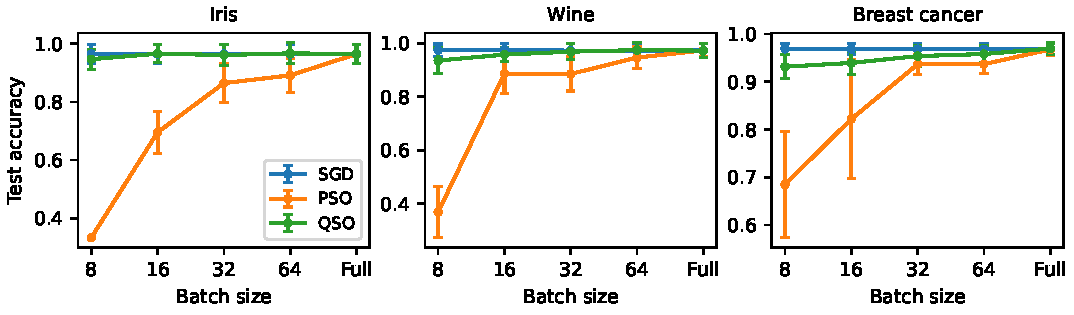
\includegraphics[width=\textwidth]{figures/acc_vs_batch.pdf}
\caption{Mean test accuracy against batch size}
\label{fig:batch}
\end{figure*}

PSO depended strongly on the batch size. For the Iris problem, the
mean accuracy of PSO rose from 0.333 at a batch size of eight to
0.964 at full batch. QSO showed the same trend in a much weaker form.
On the breast cancer problem, the mean accuracy of QSO rose from 0.932
at a batch size of eight to 0.970 at full batch. SGD stayed between
0.968 and 0.969 on the same problem. On breast cancer, QSO was significantly 
less accurate than SGD at all four mini-batch sizes. On Iris, QSO was 
significantly less accurate only at a batch size of eight, and on Wine only 
at batch sizes of eight and 16.

This trend agrees with the finding of Dennis \textit{et al.} that smaller 
batches cause greater changes in the error surface \cite{dennis2021}. A 
smaller batch therefore creates a more challenging dynamic problem. Since 
PSO has no mechanism for handling these changes, it performed worst at the 
smallest batch sizes.

The full-batch case provided a static control. Here, the error surface 
remained unchanged, so QSO's re-evaluation step had no effect. QSO and PSO 
showed no significant difference in this static case, despite QSO still 
using quantum particles. This suggests that the advantage of QSO under 
mini-batching came from its ability to respond to the changing error surface.

\subsection{Convergence Behaviour}
Figure~\ref{fig:conv} shows the median validation cross-entropy during
training for a batch size of eight and for full batch.

\begin{figure*}[t]
\centering
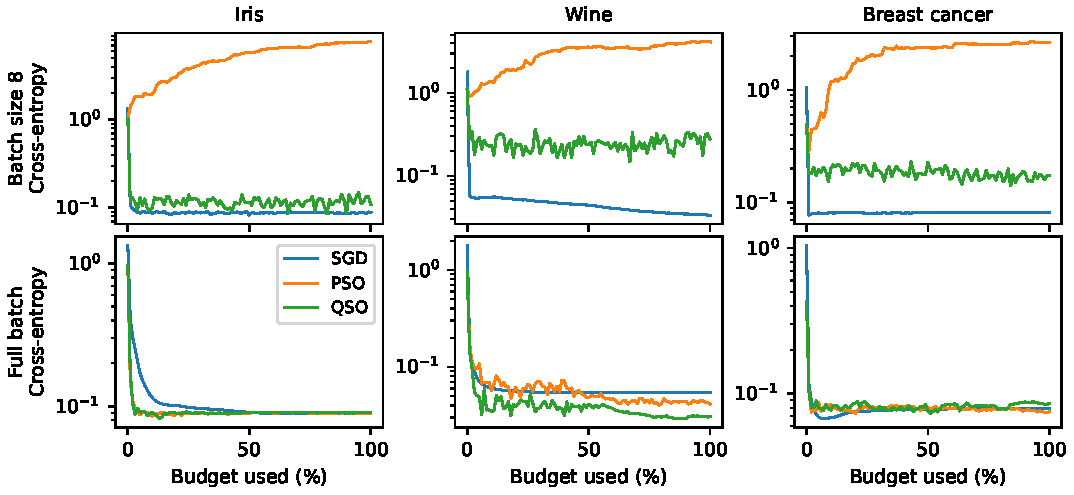
\includegraphics[width=\textwidth]{figures/convergence.pdf}
\caption{Validation cross-entropy during training}
\label{fig:conv}
\end{figure*}

At a batch size of eight, the validation cross-entropy of PSO
increased during training on all three problems. The increase was caused by
outdated memory. PSO never re-evaluated the stored best positions. An error value computed on
one mini-batch was therefore compared with errors computed on other
mini-batches.

With only eight patterns, a weight vector sometimes fit one
mini-batch almost perfectly. The weight vector then became the global
best position, even when the weight vector performed poorly on the
rest of the data. Only a position with an even lower error on a
single mini-batch replaced the global best position. The swarm was
therefore pulled towards weight vectors that fit individual
mini-batches, and the validation error grew over time.

QSO did not show this behaviour. Its validation cross-entropy dropped quickly 
at the start of training before reaching a relatively stable level. 
Re-evaluating the personal best positions on each new mini-batch kept the 
swarm's memory up to date, while the quantum particles maintained diversity 
by remaining spread around the global best position. At a batch size of 
eight, the QSO curve was more noisy because the global best was recalculated 
for every new mini-batch.

QSO still reached a higher validation error than SGD at a batch size of eight. 
SGD used the gradient of the error to move downhill on each mini-batch, 
whereas QSO relied only on error values and random sampling within the 
quantum cloud. Dennis \textit{et al.} suggested that dynamic optimisers could 
be modified to use the gradient information available during NN training \cite{dennis2021}. The 
results of this study support this suggestion. With full-batch training, all 
three algorithms converged to similar validation errors across all three 
problems.

\subsection{Outcome of the Hypothesis}
The hypothesis stated that an optimiser developed for dynamic
problems is the best choice to train NNs under mini-batching. The
results partly supported the hypothesis. QSO won all 12 mini-batch
comparisons against PSO on accuracy, and the difference disappeared
at full batch. Handling mini-batch training as a dynamic problem
therefore improved swarm-based training. However, QSO never
outperformed SGD and was significantly less accurate than SGD in
seven cases. The claim that a dynamic optimiser is the best choice
was therefore not supported for the problems, batch sizes and control
parameters used.

In summary, SGD produced the best results on all three problems. QSO
clearly outperformed PSO under mini-batching and matched the accuracy
of SGD on the Iris and Wine problems at batch sizes of 32 and larger.

% ============================================================
\section{Conclusions}
\label{sec:concl}
This study investigated whether an optimiser designed for dynamic problems is 
better suited to training neural networks (NNs) under mini-batching. 
Stochastic gradient descent (SGD), the standard inertia particle swarm 
optimiser (PSO), and the quantum-inspired particle swarm optimiser (QSO) 
were compared across three classification problems and five batch sizes.

QSO significantly outperformed PSO in every mini-batch case for accuracy, 
while this difference disappeared with full-batch training. PSO performed 
poorly at small batch sizes because its outdated personal and global best 
positions kept the swarm focused on weight vectors that fitted previous 
mini-batches. QSO addressed this through re-evaluation and the use of 
quantum particles. However, SGD achieved the best results on all three 
problems, and QSO did not outperform it. The hypothesis was therefore 
supported only when comparing the dynamic and static swarm approaches.

% ============================================================
\begin{thebibliography}{99}

\bibitem{blackwell2006}
T. Blackwell and J. Branke, ``Multiswarms, exclusion, and
anti-convergence in dynamic environments,'' \textit{IEEE Transactions
on Evolutionary Computation}, vol. 10, no. 4, pp. 459--472, 2006.

\bibitem{dennis2021}
C. Dennis, A. P. Engelbrecht, and B. M. Ombuki-Berman, ``An analysis
of the impact of subsampling on the neural network error surface,''
\textit{Neurocomputing}, vol. 466, pp. 252--264, 2021.

\bibitem{engelbrecht2007}
A. P. Engelbrecht, \textit{Computational Intelligence: An
Introduction}, 2nd ed. Chichester, UK: John Wiley \& Sons, 2007,
pp. 289--291, 303--304, 306, 311--314, 337--339, 346--348, 354--355.

\bibitem{friedman1940}
M. Friedman, ``A comparison of alternative tests of significance for
the problem of $m$ rankings,'' \textit{The Annals of Mathematical
Statistics}, vol. 11, no. 1, pp. 86--92, 1940.

\bibitem{goodfellow2016}
I. Goodfellow, Y. Bengio, and A. Courville, \textit{Deep Learning}.
Cambridge, MA: MIT Press, 2016, pp. 226--230, 249.

\bibitem{holm1979}
S. Holm, ``A simple sequentially rejective multiple test procedure,''
\textit{Scandinavian Journal of Statistics}, vol. 6, no. 2,
pp. 65--70, 1979.

\bibitem{kelleher2015}
J. D. Kelleher, B. Mac Namee, and A. D'Arcy, \textit{Fundamentals of
Machine Learning for Predictive Data Analytics: Algorithms, Worked
Examples, and Case Studies}. Cambridge, MA: MIT Press, 2015,
pp. 92--93, 335--343, 357, 400--401, 405--406, 414--417.

\bibitem{wilcoxon1945}
F. Wilcoxon, ``Individual comparisons by ranking methods,''
\textit{Biometrics Bulletin}, vol. 1, no. 6, pp. 80--83, 1945.

\end{thebibliography}

\end{document}